\documentclass[a4paper,12pt]{article}

\usepackage{graphicx}
\usepackage{amsmath}
\usepackage{array}
\usepackage{booktabs}
\usepackage{hyperref}
\usepackage{float}
\title{\textbf{Scientific Calculator using Arduino}}
\author{Prajwal\\EE24BTECH11051}
\date{\today}

\begin{document}

\maketitle
\newpage
\tableofcontents

\newpage

\section{Introduction}
\begin{itemize}
    \item Scientific calculator is used for mathematically functions like trignometric,logarithms,exponential and arithmetic.
    \item In this project we mainly try to implement the logics and computational ability of an scientific calculator using arduino board,a 16x2 LCD display and a button matrix for numericals and functions
    \item Following are the logics to implement the calculation of the mathematical functions efficently and accurately
    \begin{itemize}
        \item CORDIC algorithm for trignometric functions
        \item RK4 for logorithm and exponential 
        \item Common math operators for arithmetic operator
    \end{itemize}
\end{itemize}

\section{Components}
The following bullet points provides the components and their function briefly

\begin{itemize}
    \item \textbf{Arduino Uno -} \ Used as the brain of the calculator which uploads and recieves the input and and send cammands to display the expression and output in LCD display
    \item \textbf{16x2 LCD display -} \ displays the input and output 
    \item \textbf{Buttons Matrix -} \ Buttons are used for giving input in which we assign a character to each button. \\
    There are two modes for each button,
    \begin{itemize}
        \item Mode 1 - for numbers and basic arithmetic operations
        \item Mode 2 - for mathematical functions trignometric,logorithmic etc
    \end{itemize}
    And a button to switch between the modes
    \item \textbf{Resistors and Wires -} \ Resistor for controlling the current and wires for connections
    \item \textbf{Potentiometer -} \ For controlling the contrast of the LCD display
\end{itemize}
\begin{table}[H]
    \centering
    \renewcommand{\arraystretch}{1.2} % Adjust row height
    \begin{tabular}{|c|c|}
        \hline
        \textbf{Component} & \textbf{Arduino Pin} \\
        \hline
        \multicolumn{2}{|c|}{\textbf{Button Matrix}} \\
        \hline
        Row 1 & 2 \\
        Row 2 & 3 \\
        Row 3 & 4 \\
        Row 4 & 5 \\
        Column 1 & 6 \\
        Column 2 & 7 \\
        Column 3 & 8 \\
        Column 4 & 9 \\
        Column 5 & 10 \\
        \hline
        \multicolumn{2}{|c|}{\textbf{Shift Button}} \\
        \hline
        Shift Button & 13 \\
        GND & GND \\
        \hline
        \multicolumn{2}{|c|}{\textbf{LCD Display (16x2, Non-I2C)}} \\
        \hline
        LCD RS & A0 \\
        LCD EN & A1 \\
        LCD D4 & A2 \\
        LCD D5 & A3 \\        
        LCD D6 & A4 \\
        LCD D7 & A5 \\
        \hline
    \end{tabular}
    \caption{Circuit Connections of the Scientific Calculator}
    \label{tab:circuit_connections}
\end{table}
\newpage

\begin{figure}[H]
    \centering
    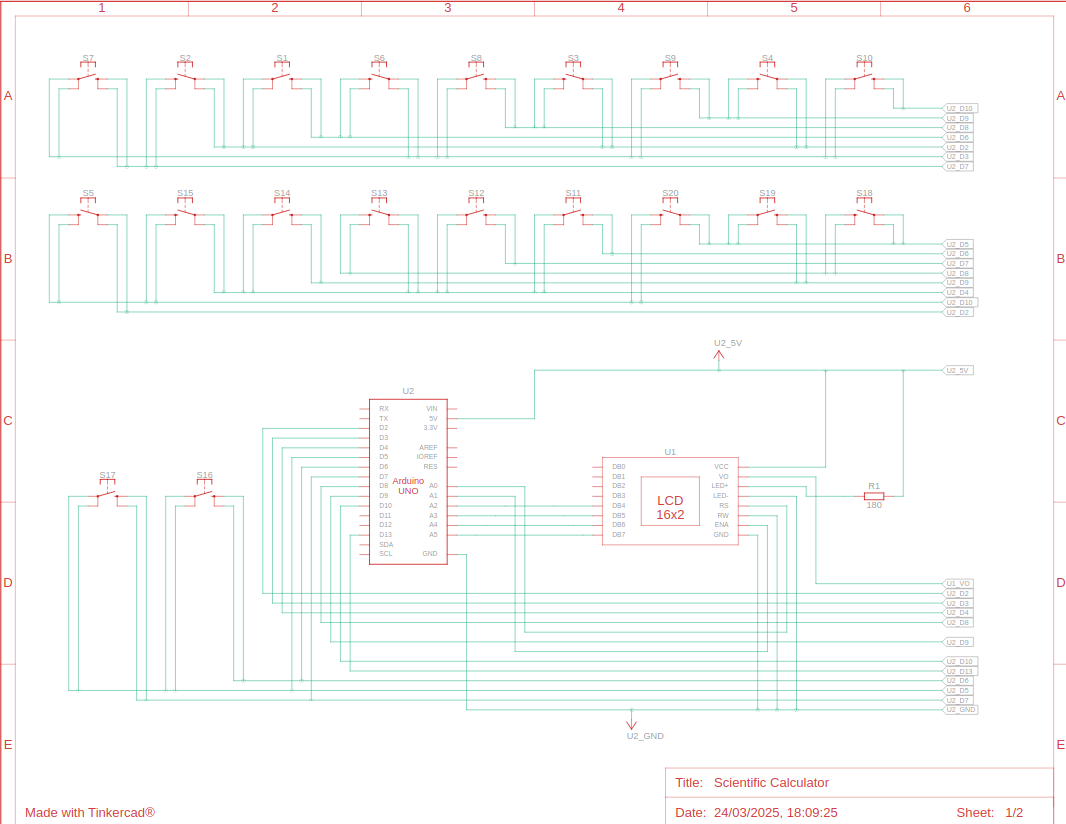
\includegraphics[width=\textwidth]{figs/circuit1.png}
    \caption{Circuit Diagram of the Scientific Calculator (Sheet 1)}
    \label{fig:circuit1}
\end{figure}

\begin{figure}[H]
    \centering
    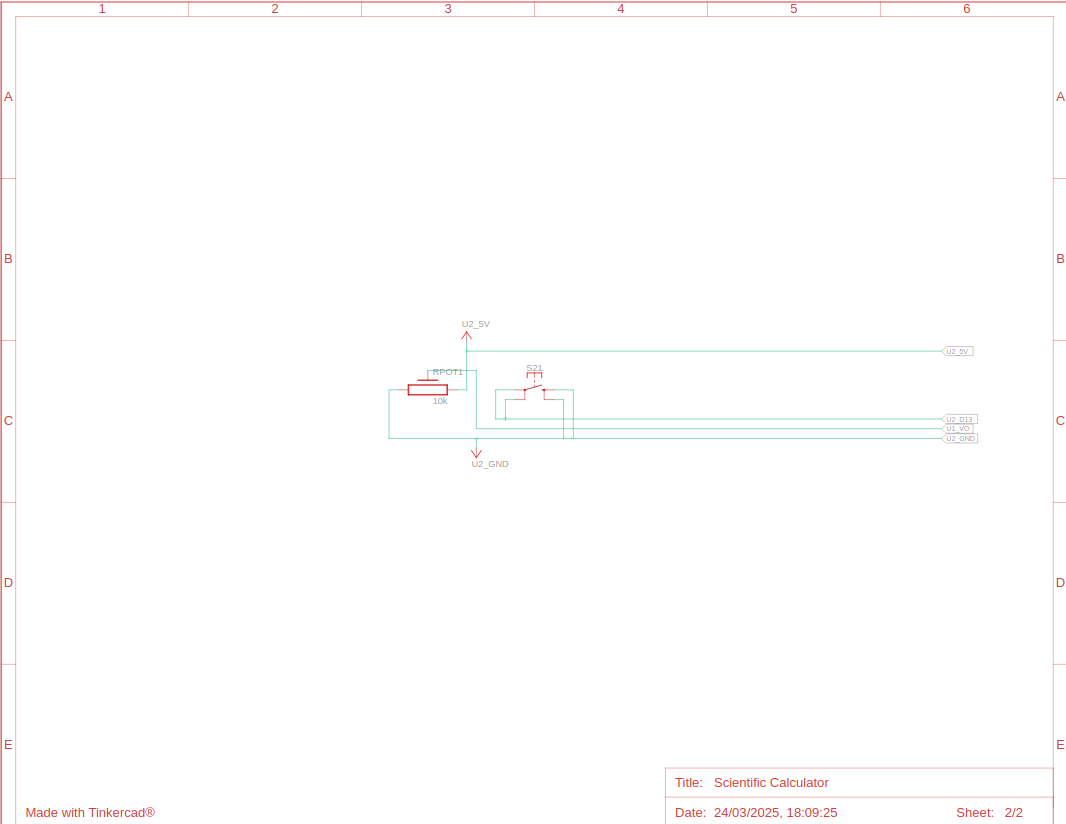
\includegraphics[width=\textwidth]{figs/circuit2.png}
    \caption{Circuit Diagram of the Scientific Calculator (Sheet 2)}
    \label{fig:circuit2}
\end{figure}

\section{Functions Available}
The calculator supports following mathematical operations.

\subsection{Mode-1 Button Layout}
\begin{table}[h]
    \centering
    \begin{tabular}{|c|c|c|c|c|}
        \hline
        1 & 2 & 3 & / & C \\
        \hline
        4 & 5 & 6 & * & D \\
        \hline
        7 & 8 & 9 & - & ( \\
        \hline
               . & 0 & = & + & ) \\
        \hline
    \end{tabular}
    \caption{Mode-1 button layout}
    \label{tab:normal_buttons}
\end{table}

\subsection{Mode-2 Button Layout}
\begin{table}[h]
    \centering
    \begin{tabular}{|c|c|c|c|c|}
        \hline
        $\sin$ & $\cos$ & $\tan$ & $x^y$ & C \\
        \hline
        ! & $\pi$ & $e$ & $|x|$ & D \\
        \hline
        log & ln & sqrt & cbrt & r \\
        \hline
        $sin^{-1}$ & $cos^{-1}$ & $tan^{-1}$ & $x^2$ & $x^3$ \\
        \hline
    \end{tabular}
    \caption{Mode button layout}
    \label{tab:shift_buttons}
\end{table}

\newpage

\section{Numerical Methods}
For accuracy and efficency the calculator uses the following numerical methods
\begin{itemize}
    \item \textbf{CORDIC Algorithm for Trignometric funtions}\\
\[
    x_{i+1} = x_i - d_i \cdot y_i \cdot 2^{-i}
    \]
    \[
    y_{i+1} = y_i + d_i \cdot x_i \cdot 2^{-i}
    \]
    \[
    z_{i+1} = z_i - d_i \cdot \text{atan}(2^{-i})
\]
where:
\begin{itemize}
    \item \( x, y \) represent the coordinates of the rotated vector.
    \item \( z \) is the angle being processed.
    \item \( d_i \) is the sign of \( z \).
\end{itemize}
It used for sin(x),cos(x) and tan(x).
\item \textbf{RK4 Algorithm for logarithmic and power functions}\\
\[
k_1 = h f(x_n, y_n)
\]
\[
k_2 = h f(x_n + \frac{h}{2}, y_n + \frac{k_1}{2})
\]
\[
k_3 = h f(x_n + \frac{h}{2}, y_n + \frac{k_2}{2})
\]
\[
k_4 = h f(x_n + h, y_n + k_3)
\]
\[
y_{n+1} = y_n + \frac{1}{6} (k_1 + 2k_2 + 2k_3 + k_4)
\]
Applications in the calculator 
\begin{itemize}
    \item \textbf{Logarithms}
    \item \textbf{Exponential}
    \item \textbf{Square and Cube Roots}
    \item \textbf{Inverse Trignometric Functions}
\end{itemize}
\end{itemize}
\section{Expression Evaluation Logic}
To handle complex expressions, the calculator uses:
\begin{itemize}
    \item **Stack-based computation**: Uses two stacks for values and operators.
    \item **Operator precedence rules**: Implements precedence to ensure correct order of operations.
    \item **String parsing**: Extracts numbers, operators, and function names.
    \item **Error handling**: Handles division by zero and invalid inputs.
\end{itemize}

\section{Implementation Challenges and Solutions}
\begin{itemize}
    \item **Handling Button Multiplexing**: Since the number of input pins is limited, a multiplexing technique was used to read button presses efficiently.
    \item **Non-I2C LCD Handling**: The LCD was operated in 4-bit mode to optimize pin usage.
    \item **Efficient Mathematical Computation**: Using CORDIC and RK4 improved accuracy while reducing computation time.
\end{itemize}

\section{Conclusion}
\begin{itemize}
    \item This scientific calculator successfully implements a variety of mathematical functions using efficient numerical methods. The combination of CORDIC and RK4 ensures accurate and fast computations.
    \item The button matrix provides an intuitive interface, making it a practical and functional scientific calculator.
\end{itemize}
For codes refer\\
\url{https://github.com/naraprajwal/EE1003/tree/ee654ce2686dc1c07586fa8eb6452a7e21e719c8/Calculator/codes}\\

\centering
Thank you

\end{document}
